\documentclass{scrartcl}
\usepackage[utf8]{inputenc}
\usepackage{graphicx}
\usepackage{geometry}
\usepackage{titling}
\usepackage{listings}
\usepackage{amsmath}

% Configuration
\graphicspath{ {img/} }
\geometry{a4paper}
\lstset{basicstyle=\footnotesize\ttfamily,breaklines=true}
\lstset{framextopmargin=50pt}

\renewcommand\partheadstartvskip{\clearpage\null\vfil}
\renewcommand\partheadmidvskip{\par\nobreak\vskip 20pt\thispagestyle{empty}}
\renewcommand\partheadendvskip{\vfil\clearpage}
\renewcommand\raggedpart{\centering}


% Title
\title{Yet Another Stupid Compiler}
\author{
    Louis Solofrizzo\\
    \texttt{louis@ne02ptzero.me}\\
    \\
    42 Staff\\
    \texttt{staff@42.fr}
}

\pretitle{%
    \begin{center}
    \LARGE
    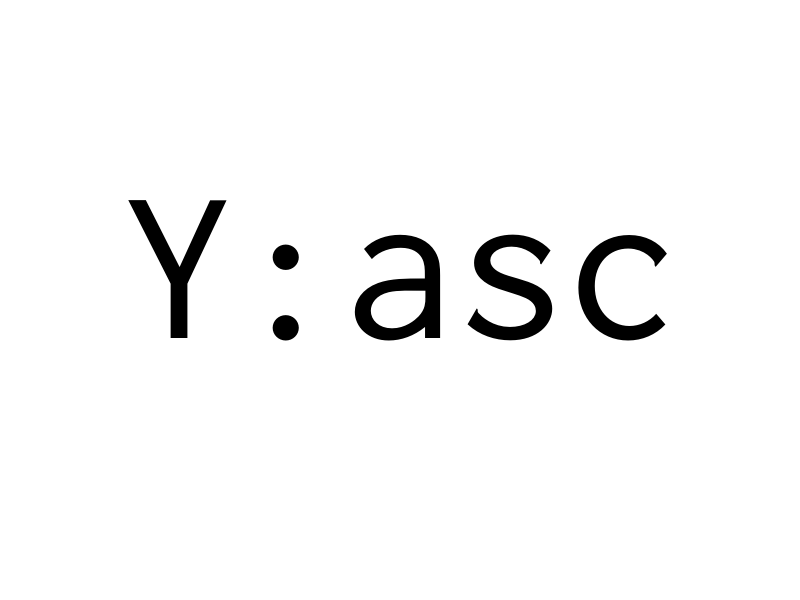
\includegraphics[scale=0.1, height=7cm]{logo}\\[\bigskipamount]
}

\posttitle{%
    \end{center}
}


% Actual document
\begin{document}

\begin{titlingpage}
    \maketitle
\end{titlingpage}


    \tableofcontents{}
    \newpage

\part{Introduction}
\part{The Y Language}
    \section{The basics}
        \subsection{File format}
            All files in the Y programming language will have the \texttt{.y}
            extension. Though this extension serve no purpose, we advise the
            reader to stick to this rule, as is it much better for organizing files.
        \subsection{Instructions}
            In the Y language, one must declare an instruction with a \texttt{;}
            at the end of it
            \begin{lstlisting}
    instruction;
            \end{lstlisting}
            One can chain instruction on the same line, regardless of line breaks
            \begin{lstlisting}
    instruction1; instruction2;
            \end{lstlisting}
            It is worth noting that the Y language does not care about line returns,
            in whatever standards (\textbackslash n, \textbackslash r\textbackslash n, ..)
        \subsection{Scope}
            As many programming languages, Y use a couple of brackets \texttt{\{\}}
            to determine scope. Scope is to be determined on special instructions,
            like conditions, functions and namespaces.
            \begin{lstlisting}
    if (condition) {
        /* If's scope */
    }

    [...]

    function(ubyte[] : str) : bool {
        /* Function's scope */
    }
            \end{lstlisting}
            One can use brackets to determine an internal scope, that serve no
            other purpose that limiting variable use
            \begin{lstlisting}
    {
        u32 num = 2;

        print("Num is equal to %u\n", num);
    }
    /* Cannot use num here */
            \end{lstlisting}

        \subsection{Comments}
            Comments can be written in the following format
            \begin{lstlisting}
    /* Comment here */
            \end{lstlisting}
            Those are only for the developer, as it will not be compiled.

    \section{Types, Operators and Expressions}
        Variables and constants are the basic data objects manipulated in a
        program. Declarations list the variables to be used, and state what type
        they have and perhaps what their inititial values are. Operators
        specify what is to be done with them. Expressions combine variables and
        constants to produce new values. The type of an object determines the set
        of values it can have and what operations can be performed on it. These
        building blocks are the topic of this chapter.

        \subsection{Declarations}
            All variables must be declared before use, although certain
            declarations can be made implicity by content. A declaration
            specifies a type, an optionnal flag and a name.
            \begin{lstlisting}
    u32                 count, j;
    bool __const        ret = true;
            \end{lstlisting}
            Variables can be distributed among declarations in any fashion; the
            list above could well be written as
            \begin{lstlisting}
    u32         count;
    u32         j;
            \end{lstlisting}
            A variable may also be initialized in its declaration. If the name
            is followed by an equals signs and an expression, the expression
            serves as an initializer. Constant variables must be initialized,
            see the \ref{const} section for more information.

            The flag between the type and the name is implemented by the language,
            and should always be in this position.
        \subsection{Arithmetic Operators}
            The binary arithmetic operators are \texttt{+}, \texttt{-},
            \texttt{*}, \texttt{/} and the modulus operator \texttt{\%}.
            The binary operator \texttt{+} and \texttt{-} operators have the 
            same precedence, which is lower than the precedence of \texttt{*},
            \texttt{/}, and \texttt{\%}. Arithmetic operators associate left
            to right.

        \subsection{Variable names} \label{varnames}
            Variable names are made up of letters and digits; the first character
            must be a letter. A letter is, in this context, a character inside
            the English dictionnary, through the letters \texttt{a} to \texttt{z}.
            All other symbols from other languages / Unicode are not supported,
            and will throw an error upon reading. The underscore \texttt{\_}
            count as a letter. All variable must be in lowercase, as uppercase
            names are reserved to namespaces.
            Keywords like \texttt{if}, \texttt{else}, \texttt{struct}, etc., are
            reserved: They cannot be used as variables names.

            A variable name cannot be used twice in a scope: If such a thing
            would happen, an error will be thrown. However, different variables
            can have the same name in differents namespaces. See the \ref{namespaces}
            section for more information.
        \subsection{Data types and Sizes}
            One can use the following standard data types:

$\begin{array}{|c|c|c|}
\hline
Name & Range & Content\\
\hline
\text{ubyte} & \text{0 - 255} & \text{One byte, can be used for an ASCII-character}\\
\hline
\text{u8} & \text{0 - 255} & \text{Unsigned integer on 8 bits, same as ubyte}\\
\hline
\text{s8} & \text{-128 - 127} & \text{Signed integer on 8 bits}\\
\hline
\text{u16} & \text{0 - 65,535} & \text{Unsigned integer on 16 bits}\\
\hline
\text{s16} & \text{-32,768 - 32,767} & \text{Signed integer on 16 bits}\\
\hline
\text{u32} & \text{0 - 4,294,967,295} & \text{Unsigned integer on 32 bits}\\
\hline
\text{s32} & \text{-2,147,483,648 - 2,147,483,647} & \text{Signed integer on 32 bits}\\
\hline
\end{array}$
        \subsection{Constants} \label{const}
            One can declare a specific variable to never be changed, in any scope,
            via the keyword \texttt{\_\_const}:
            \begin{lstlisting}
    ubyte __const char = 'A';
            \end{lstlisting}
            This \texttt{char} variable can never change value; any attempt to it
            will throw an error.
            Constant variables must have a initialization value, otherwise, its
            utility is quite limited.

            The \texttt{\_\_const} keyword must always be between a variable
            type and its name.

        \subsection{Inline Constant Declarations}
            One can use inline constant declarations in order to simplify code
            \begin{lstlisting}
    print("Hello!");
            \end{lstlisting}
            Here, the \texttt{Hello!} is a constant inline string. One can also
            use an integer constant like \texttt{1234}, which is by default an
            unsigned integer on 32 bits; therefore, the following example is wrong
            \begin{lstlisting}
        print_int(u8 : num) : void {
            print("%d\n", num);
        }

        [...]

        main(u32 : ac, ubyte[]* : av) : u32 {
            print_int(23);
        }
            \end{lstlisting}
            Instead, one must use
            \begin{lstlisting}
        print_int(u32_to_u8(23));
            \end{lstlisting}
            Which is valid by the type conversions standard of the Y language, see
            \ref{Type_conv} section for more information.

            In order to gain some performance at run-time, by avoiding a function call,
            one can use constants cast
            \begin{lstlisting}
        print_int(__u8(23));
            \end{lstlisting}
            It will change the internal type of the variable at compilation time,
            acting like a cast. See the \ref{comp_cast} section for more information.

            The value of an integer can be specified in octal or hexadecimal
            instead of decimal. A leading \texttt{0} (zero) on an integer
            constant means octal; a leading \texttt{0x} or \texttt{0X} means
            hexadecimal.  For example, decimal 31 can be written as
            \texttt{037} in octal and \texttt{0x1f} or \texttt{0x1F} in hex.

            A character constant is an integer, written as one character within
            single quotes, such as \texttt{'x'}. The value of a character constant
            is the numeric value of the characters in the machine's character set.
            For example, in the ASCII character set the character constant \texttt{'0'}
            has the value \texttt{48}, which is unrelated to the numeric value \texttt{0}.

            Certain characters can be represented in character and string constants
            by escape sequences like \texttt{\textbackslash n} (newline); these sequences look
            like two characters, but represent only one. In addition, an arbitrary
            byte-sized (ubyte) pattern can be specified by
            \begin{lstlisting}
        '\ooo'
            \end{lstlisting}
            Where \texttt{ooo} is one to three octal digits (0..7) or by
            \begin{lstlisting}
        '\xhh'
            \end{lstlisting}
            where \texttt{hh} is one or more hexadecimal digits (0..9, a..f, A..F).
            The complete set of escape sequences is
\\\\
$\begin{array}{|l|l|}
\hline
Sequence & Value\\
\hline
\backslash a & \text{alert (bell) character} \\
\hline
\backslash b & \text{backspace} \\
\hline
\backslash f & \text{formfeed} \\
\hline
\backslash n & \text{newline} \\
\hline
\backslash r & \text{carriage return} \\
\hline
\backslash t & \text{horizontal tab} \\
\hline
\backslash v & \text{vertical tab} \\
\hline
\backslash \backslash & \text{backslash} \\
\hline
\backslash ? & \text{question mark} \\
\hline
\backslash ' & \text{single quote} \\
\hline
\backslash " & \text{double quote} \\
\hline
\backslash ooo & \text{octal number} \\
\hline
\backslash xhh & \text{hexadecimal number} \\
\hline
\end{array}$
\\\\
        The character constant \texttt{'\textbackslash 0'} represents the character
        with value zero, the null character.

        A \texttt{constant expression} is an expression that involves only constants.
        Such expressions may be evaluated at during compilation rather than run-time,
        and accordingly may be used in any place that a constant occur, as in
        \begin{lstlisting}
    ubyte[100 + 20]     str;
        \end{lstlisting}
        will be compiled as
        \begin{lstlisting}
    ubyte[120]     str;
        \end{lstlisting}

        A string constant, or string literal, is sequence of zero or more
        characters surrounded by doubles quotes, as in
        \begin{lstlisting}
    "I am a string"
        \end{lstlisting}
        or
        \begin{lstlisting}
    "" /* The empty string */
        \end{lstlisting}
        The quotes are not part of the string, but serve only to delimit it. The
        same escape sequences used in character constants apply in strings;
        \textbackslash " represents the double-quote character. String constants
        can be concatenated at compile time:
        \begin{lstlisting}
    "hello, " "world"
        \end{lstlisting}
        is equivalent to
        \begin{lstlisting}
    "hello, world"
        \end{lstlisting}

        \subsection{Relational and Logical Operators}
            The relational operators are

$\begin{array}{llll}
> & >= & < & <=
\end{array}$

            They all have the same precedence. Just below them in precedence are
            the equality operators:

$\begin{array}{ll}
== & !=
\end{array}$

            Relational operators have lower precedence than arithmetic operators,
            so an expression like \texttt{i < lim - 1} is taken as \texttt{i < (lim - 1)}
            , as would be expected.

            The logical operators are

$\begin{array}{ll}
\&\& & ||
\end{array}$

            Expressions connected by \texttt{\&\&} or \texttt{||} are evaluated
            left to right, and evaluation stops as soon as the truth or falsehood
            of the result is known. By definition, the numeric value of a relational
            or logical expression is 1 if the relation is true, and 0 if the relation
            is false.

        \subsection{Type Conversions} \label{Type_conv}
            In the Y language, there is no such thing as 'implicit type conversion':
            All conversions must be explicit, using the standard functions.
            Therefore, the following example is wrong:
            \begin{lstlisting}
                u32     i = 10;
                u8      j;

                i = j;
            \end{lstlisting}
            In place of that, one must use
            \begin{lstlisting}
                u32     i = 10;
                u8      j;

                j = u32_to_u8(i);
            \end{lstlisting}
            All standards type-conversions function are to be safe, with no
            possibilty of underflow or overflow. You can find all the standards
            function below:
\\\\
\hspace*{-60px}
$\begin{array}{|l|l|l|l|}
\hline
Name & Argument & Returns & Role\\
\hline
\text{u8\_to\_u16} & \text{u8} & \text{u16} & \text{Convert an unsigned integer on 8 bits to an unsigned integer on 16 bits}\\
\hline
\text{u8\_to\_u32} & \text{u8} & \text{u32} & \text{Convert an unsigned integer on 8 bits to an unsigned integer on 32 bits}\\
\hline
\text{u16\_to\_u8} & \text{u16} & \text{u8} & \text{Convert an unsigned integer on 16 bits to an unsigned integer on 8 bits}\\
\hline
\text{u16\_to\_u32} & \text{u16} & \text{u32} & \text{Convert an unsigned integer on 16 bits to an unsigned integer on 32 bits}\\
\hline
\text{u32\_to\_u8} & \text{u32} & \text{u8} & \text{Convert an unsigned integer on 32 bits to an unsigned integer on 8 bits}\\
\hline
\text{u32\_to\_u16} & \text{u32} & \text{u16} & \text{Convert an unsigned integer on 32 bits to an unsigned integer on 16 bits}\\
\hline
\text{s8\_to\_s16} & \text{s8} & \text{s16} & \text{Convert a signed integer on 8 bits to a signed integer on 16 bits}\\
\hline
\text{s8\_to\_s32} & \text{s8} & \text{s32} & \text{Convert a signed integer on 8 bits to a signed integer on 32 bits}\\
\hline
\text{s16\_to\_s8} & \text{s16} & \text{s8} & \text{Convert a signed integer on 16 bits to a signed integer on 8 bits}\\
\hline
\text{s16\_to\_s32} & \text{s16} & \text{s32} & \text{Convert a signed integer on 16 bits to a signed integer on 32 bits}\\
\hline
\text{s32\_to\_s8} & \text{s32} & \text{s8} & \text{Convert a signed integer on 32 bits to a signed integer on 8 bits}\\
\hline
\text{s32\_to\_s16} & \text{s32} & \text{s16} & \text{Convert a signed integer on 32 bits to a signed integer on 16 bits}\\
\hline
\end{array}$

        \subsection{Compilation time casts} \label{comp_cast}
            In order to respect the 'non implicit cast' rule on constant expressions,
            one must use standards function for it:
            \begin{lstlisting}
        print_int(u8 : num) : void {
            print("%d\n", num);
        }

        [...]

        main(u32 : ac, ubyte[]* : av) : u32 {
            print_int(u32_to_u8(23));
        }
            \end{lstlisting}
            Alternatively, in order to gain on performance, one can specify
            the desired type for the compiler:
            \begin{lstlisting}
        print_int(__u8(23));
            \end{lstlisting}
            The following keywords can be used
\\\\
$\begin{array}{l}
\_\_u8\\
\_\_ubyte\\
\_\_u16\\
\_\_u32\\
\end{array}$
\\\\
        \subsection{Precedence and Order of Evaluation}
            You can find the order of evaluation of all Y keywords below
\\\\
$\begin{array}{|l|l|}
\hline
Operators & Associativity\\
\hline
\text{() [] .} & \text{Left to right}\\
\hline
\text{! *(variable)} & \text{Right to left}\\
\hline
\text{* / \%} & \text{Left to right}\\
\hline
\text{+ -} & \text{Left to right}\\
\hline
< <= > >= & \text{Left to right}\\
\hline
\text{\&\&} & \text{Left to right}\\
\hline
|| & \text{Left to right}\\
\hline
\text{\_\_keyword()} & \text{Left to right}\\
\hline
\end{array}$
    \section{Control Flow}
        The control-flow of a language specify the order in which computations
        are performed. We have already met the most common control-flow constructions
        in earlier examples; here we will complete the set, and be more precise
        about the ones discussed before.
        \subsection{If-Else}
            The \texttt{if-else} statement is used to express decisions. Formally
            the syntax is
            \begin{lstlisting}
    if (expression)
        statement1
    else
        statement2
            \end{lstlisting}
            where the else part is optional. The \texttt{expression} is evaluated;
            if it is true (that is, if \texttt{expression} has a non-zero value),
            \texttt{statement1} is executed. If it is false, (\texttt{expression} is zero)
            and there is an else part, \texttt{statement2} is executed instead.

            Since an \texttt{if} test the numeric value of an expression, certain
            shortcuts are possible. The most obvious is writing
            \begin{lstlisting}
    if (expression)
            \end{lstlisting}
            instead of
            \begin{lstlisting}
    if (expression != 0)
            \end{lstlisting}
            Because the \texttt{else} part on an \texttt{if-else} is optionnal,
            there is ambiguity when an else if ommited from a nested \texttt{if}
            sequence. This is resolved by associating the \texttt{else} with
            the closest previous \texttt{else}-less \texttt{if}. For example, in
            \begin{lstlisting}
    if (n > 0)
        if (a > b)
            z = a;
        else
            z = b;
            \end{lstlisting}
            the \texttt{else} goes to the inner \texttt{if}, as we have shown by
            indentation. If that isn't the desired behaviore, one must use braces
            to force the proper association:
            \begin{lstlisting}
    if (n > 0) {
        if (a > b)
            z = a;
    }
    else
        z = b;
            \end{lstlisting}

        \subsection{Else-If}
            The construction
            \begin{lstlisting}
    if (expression)
        statement;
    else if (expression)
        statement;
    else if (expression)
        statement;
    else if (expression)
        statement;
    else if (expression)
        statement;
    else
        statement;
            \end{lstlisting}
            occurs so often that is worth a brief separate discussion. This
            sequence of \texttt{if} statements is the most general way of writing
            a multi-way decision. The \texttt{expressions} are evaluated in order;
            if an \texttt{expression} is true, the \texttt{statement} associated
            with it is executed, and this terminates the whole chain. As always,
            the code for each \texttt{statement} is either a single statement,
            or a group of them in braces.

            The last \texttt{else} part handles 'none of the above' or default
            case where none of the other conditions is satisfied. Sometimes there
            is no explicit action for the default; in that case the trailing
            \begin{lstlisting}
    else
        statement;
            \end{lstlisting}
            can be ommited, or it may be used for error checking to catch an
            'impossible' condition.
        \subsection{Loops - While}
            In
            \begin{lstlisting}
    while (expression)
        statement;
            \end{lstlisting}
            the \texttt{expression} is evaluated. It it is non-zero, \texttt{statement}
            is executed and \texttt{expression} is re-evaluated. This cyccle continutes
            until \texttt{expression} becomes zero, at which point execution
            resumes after \texttt{statement}.
        \subsection{Loops - For}
            The \texttt{for} statement
            \begin{lstlisting}
    for (expr1; expr2; expr3)
        statement;
            \end{lstlisting}
            is equivalent to
            \begin{lstlisting}
    expr1;
    while (expr2) {
        statement;
        expr3;
    }
            \end{lstlisting}
            except for the behaviour of \texttt{continue}, which is described
            in section \ref{break_n_continue}.

            Grammatically, the three components of a \texttt{for} loop are
            expressions. Most commonly, \texttt{expr1} and \texttt{expr3} are
            assignements or function calls and \texttt{expr2} is a relational
            expressions. Any of the three parts can be ommited, although the 
            semicolons \texttt{;} must remain. You can find a simple example
            of a \texttt{for} usage below:
            \begin{lstlisting}
    u8          i;
    ubyte[]     str = "Hello !";

    for (i = 0; str[i] != '\0'; i++)
        print("Letter position %d is %c\n", i, str[i]);
            \end{lstlisting}
        \subsection{Loops - Do-While}
            As we discussed earlier, the \texttt{while} and \texttt{for} loops
            test the termination condition at the top. By contrast, the \texttt{do-while}
            loop tests at the bottom \texttt{after} making each pass through the 
            loop body; the body is always executed at least once.

            The syntax of the \texttt{do} is
            \begin{lstlisting}
    do
        statement;
    while (expression);
            \end{lstlisting}
            The \texttt{statement} is executed, then \texttt{expression} is
            evaluated. If it is true, \texttt{statement} is evaluated again, and so on.
            When the expression becomes false, the loop terminates.
        \subsection{Break and Continue} \label{break_n_continue}
            It is sometimes convenient to be able to exit from a loop other than
            by testing at the top or bottom. The \texttt{break} statement provides
            an early exit from \texttt{for}, \texttt{while} and \texttt{do}.
            A \texttt{break} causes the innermost enclosing loop to be exited
            immediately.

            The \texttt{continue} statement is related to \texttt{break}: it
            causes the next iteration of the enclosing \texttt{for}, \texttt{while} or
            \texttt{do} loop to begin. In the \texttt{while} and \texttt{do}, this means
            that the test part is executed immediately; in the \texttt{for}, control
            passes to the increment step.
    \section{Functions and Program Structure}
        Functions break large computing tasks into smaller ones, and enable people
        to build on what others have done instead of starting over from scratch.
        Appropriate functions hide details of operation from parts of the program
        that don't need to know about them, thus clarifying the whole, and easing
        the pain of making changes.
        \subsection{Basics}
            A function is declared like
            \begin{lstlisting}
                function_name(arguments) : return-type {
                    statement;
                }
            \end{lstlisting}
            A function is identified by its name. Function names are made up
            of letters and digits; the first character
            must be a letter. A letter is, in this context, a character inside
            the English dictionnary, through the letters \texttt{a} to \texttt{z}.
            All other symbols from other languages / Unicode are not supported,
            and will throw an error upon reading. The underscore \texttt{\_}
            count as a letter. All function must be in lowercase, as uppercase
            names are reserved to namespaces.
            Keywords like \texttt{if}, \texttt{else}, \texttt{struct}, etc., are
            reserved: They cannot be used as functions names.

            The \texttt{arguments} is a list of a variables passed to the function.
            In
            \begin{lstlisting}
                ubyte[] : str, u32 : num
            \end{lstlisting}
            The first argument, \texttt{str} is an array of \texttt{ubyte}, and
            the second one, \texttt{num}, is an unsigned integer on 32 bits.

            The \texttt{return\_type} of the function is declared after the list
            of arguments, using the character \texttt{:}. This return type
            must be respected in the function, with the \texttt{return} keyword.
            For example, the following function is wrong:
            \begin{lstlisting}
                compute_division(u32 : first, u32 : second) : u32 {
                    [...]
                    return "Hello !";
                }
            \end{lstlisting}
            since it is returning a \texttt{string}, instead of an \texttt{u32}.

            A function can take no arguments, or return nothing: in this case,
            the type \texttt{void} must be used
            \begin{lstlisting}
                function_that_does_nothing(void) : void {
                    [Nothingness...]
                }
            \end{lstlisting}
            That function can be called with
            \begin{lstlisting}
                function_that_does_nothing();
            \end{lstlisting}

        \subsection{External Variables}
        \subsection{Scope Rules}
        \subsection{Namespaces} \label{namespaces}
            Namespaces are used to limit scope of functions. They must be declared
            via the keyword \texttt{def}, with brackets to delimit the scope.
            Namespaces names are made up of letters and digits; the first character
            must be a letter, in uppercase: Lowercase names are reserved to variables.

            Example of a namespace declaration:
            \begin{lstlisting}
    def Namespace_name {
        [...]
    };
            \end{lstlisting}
            Functions can be declared in a namespace:
            \begin{lstlisting}
    def Namespace_name {
        function_name(ubyte[] : str) : bool {
            [...]
            return true;
        }
    };
            \end{lstlisting}
            Any functions declared in a namespace is meant to be used with this
            namespace. In order to use a specific namespace, one must declare it:
            \begin{lstlisting}
    use Namespace_name;
            \end{lstlisting}
            The keyword \texttt{use} used with the namespace name will allow
            the call of all functions in this namespace. In order to use one
            function of this namespace, one can use an accessor on the namespace name:
            \begin{lstlisting}
    use Namespace_name.function_name;
            \end{lstlisting}
            With this declaration, any other function of this namespace used in
            code will throw an error.

            With proper usage of the keyword \texttt{use}, one can use a
            namespace's function in the following way:
            \begin{lstlisting}
    Namespace_name.function_name("Hello!");
            \end{lstlisting}

            Since namespaces are a limited scope, they can be two functions with
            the same name, in two different namespaces but they must always be used
            with a proper accessor; this way, the compiler / interpreter will
            never be confused as what function should be called.
            However, take the following example:

            \begin{lstlisting}
    def Namespace_one {
        hello(void) : void {
            print("Hello from one");
        }
    };

    def Namespace_two {
        use Namespace_one;

        hello(void) : void {
            print("Hello from two");
            hello();
        }
    };
            \end{lstlisting}
            In the \texttt{Namespace\_two} function \texttt{hello}, we call a
            function named \texttt{hello}: In this specific case, the function
            called will be the one of the current namespace, thus resulting in
            an infinite loop. If one must use a same named function in another
            namespace, a proper accessor must be used:
            \begin{lstlisting}
    def Namespace_one {
        hello(void) : void {
            print("Hello from one");
        }
    };

    def Namespace_two {
        use Namespace_one;

        hello(void) : void {
            print("Hello from two");
            Namespace_two.hello();
        }
    };

            \end{lstlisting}
            The same logic can be used for globals functions named the same as
            namespace's function:
            \begin{lstlisting}
    hello(void) : void {
        print("Hello from one");
    }

    def Namespace_two {
        hello(void) : void {
            print("Hello from two");
            hello();
        }
    };
            \end{lstlisting}
            Here, in the \texttt{Namespace\_two.hello} function, the function
            called will be itself. However, if one call the \texttt{hello} function
            from a global scope, such as \texttt{main}, the global scope will be used:
            \begin{lstlisting}
    hello(void) : void {
        print("Hello from one");
    }

    def Namespace_two {
        hello(void) : void {
            print("Hello from two");
        }
    };

    use Namespace_two;

    main(u32 : ac, ubyte[]* : av) : u32 {
        hello();
        return 0;
    }
            \end{lstlisting}
    Will return:
            \begin{lstlisting}
    > Hello from one
            \end{lstlisting}
            If one must use the \texttt{Namespace\_two} \texttt{hello} function,
            a proper accessor must be used, as shown above.



        \subsection{Header Files}
        \subsection{Static Variables}
        \subsection{Recursion}
        \subsection{Preprocessor}
    \section{Pointers and Arrays}
        \subsection{Pointers and Addresses}
        \subsection{Pointers and Function Arguments}
        \subsection{Pointers and Arrays}
        \subsection{Address Arithmetic}
        \subsection{The \_\_heap argument}
        \subsection{Command-line Arguments}
    \section{Structures}
        \subsection{Basics}
        \subsection{Structures and Functions}
        \subsection{Array of Structures}
        \subsection{Pointer to Structures}
        \subsection{Packing}
    \section{Standard Library}
        \subsection{Input and Output}
        \subsection{Memory Control}
        \subsection{System Calls}
    \section{Format}
        \subsection{Comments}
        \subsection{Unicode}
        \subsection{Inline definitions}
\part{The ASC Language}
    \section{Getting Started}
    \section{Definitions}
    \section{Accessors}
        \subsection{Basics}
        \subsection{Special Accessors}
        \subsection{Constants}
    \section{Registers}
        \subsection{Infinite Registers}
        \subsection{Define a Register}
    \section{Memory}
        \subsection{Virtual Memory}
        \subsection{Paging}
        \subsection{On-Disk memory}
        \subsection{Cache}
    \section{Arithmetic}
        \subsection{Basics}
        \subsection{Comparisons}
        \subsection{Bit-Fields}
    \section{Calls}
        \subsection{Functions}
        \subsection{System Calls}
    \section{Format}
        \subsection{Comments}
        \subsection{Instructions}


\end{document}
